\documentclass{article}
\usepackage{tabularx}
\usepackage{amsmath}
\usepackage{here}
\usepackage{graphicx}
\usepackage[margin=2cm]{geometry}
\usepackage{cite}
\usepackage[final]{hyperref}
\usepackage{listings}
\hypersetup{
	colorlinks=true,
	linkcolor=blue,
	citecolor=blue,
	filecolor=magenta,
	urlcolor=blue         
}

\begin{document}

\title{Project\\A prey/predator simulation}
\maketitle

\section{Introduction}
The project needs to be sent four days before the final exam. Only the source code and the report are required (no binary code). Please send it to robinfaurypro@gmail.com. In the rapport, you must discuss any technical choices you did. Why you prefer to create a buffer or a surface, why you recompute this value, etc...
The project is an illustration of the Lotka Volterra simulation also known as the prey/predator model. Rabbits (in white) will randomly walk and reproduce and Foxes (in orange) will eat closest rabbits. 
\begin{figure}[H]
	\centering
	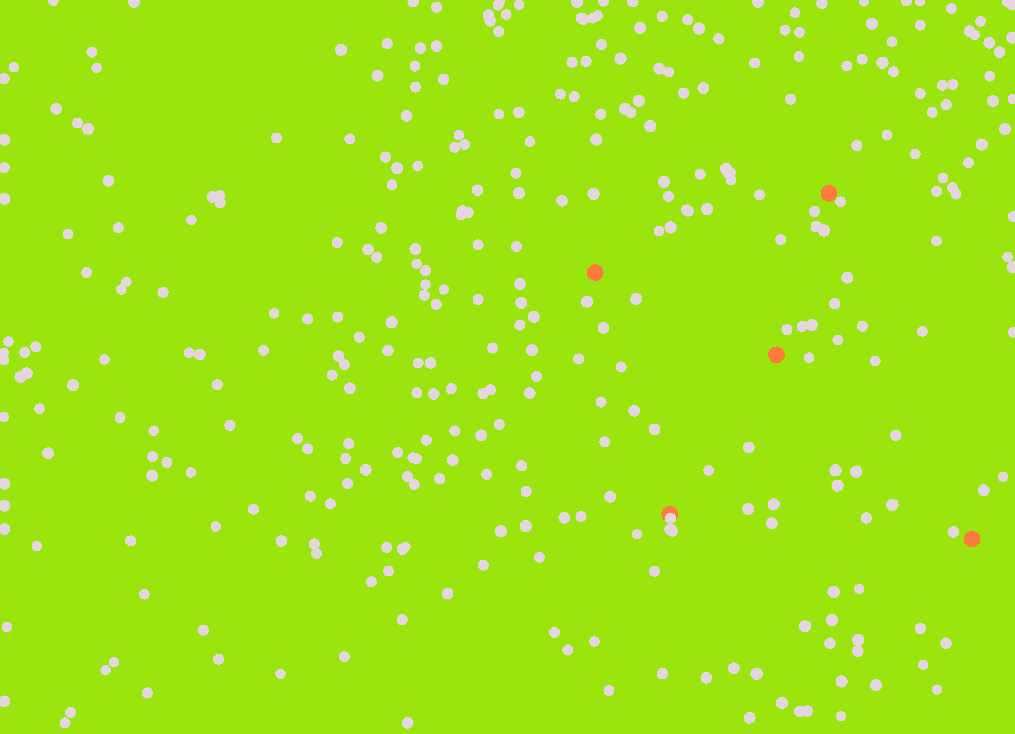
\includegraphics[scale=0.54]{figures/project.png}
	\caption{The Lotka Volterra simulation}
\end{figure}

This simulation is based on two linked differential equations.
\begin{equation}
\begin{cases}
\frac{dx(t)}{dt} = x(t)(\alpha -\beta y(t))\\
\frac{dy(t)}{dt} = y(t)(\delta x(t)-\gamma)
\end{cases}
\end{equation}
As we can see on the graph, a large amount of preys will result in a high wave of new predators. The new predator will reduce the number of preys. The simulation is very stable.
\begin{figure}[H]
	\centering
	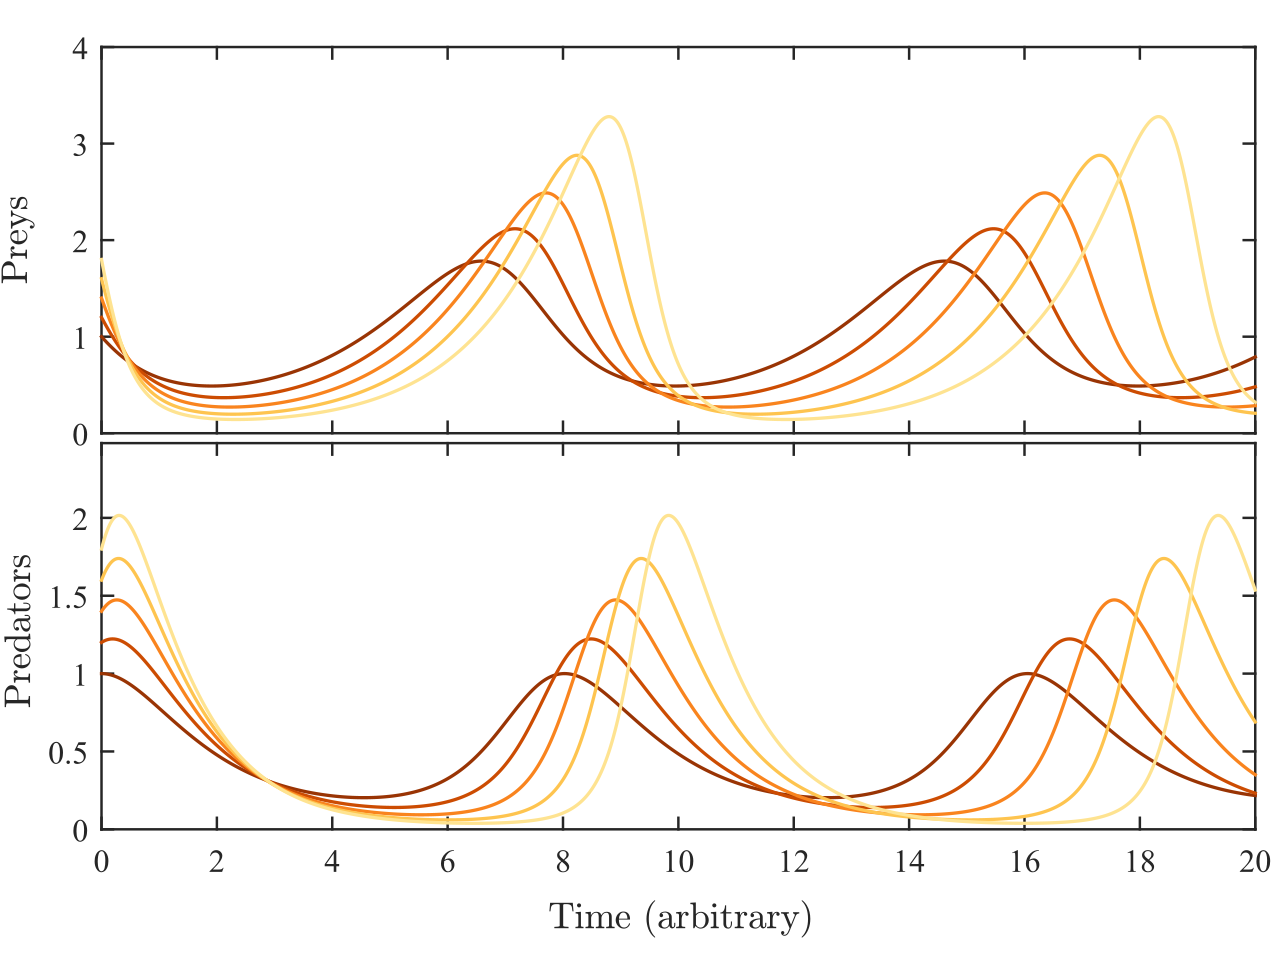
\includegraphics[scale=0.2]{figures/lotka_volterra.png}
	\caption{Graph of the equation  [Wikipedia]}
\end{figure}

\subsection{Setup}

The initial code of the project can be find in this git repository:
\begin{lstlisting}
	https://github.com/robinfaurypro/GPGPU_ISIMA_2022-2023.git
\end{lstlisting}

For this simulation, we will use a real time application. The CUDA part will compute the image to show as fast as possible and OpenGL will print this image on the screen. Working with image is more complex than working with buffer. However, to print on the screen a buffer, we need first to convert it as a texture. A better option is to work directly with texture. GPU texture can be seen in the same way than buffer, but they come with a collection of tool (interpolation, repeat, ...).\\
For this project, we ask OpenGL to generate the texture to show and we use the interop feature to convert it into a surface. Surfaces can be send to the kernel in the same way than buffers. You can create a float4 on the kernel to fill the surface with your color. You can also see how to create a surface CUDA in the example.
\begin{lstlisting}
	__global__  void kernel_draw_map(cudaSurfaceObject_t surface) {
		int32_t x = blockIdx.x * blockDim.x + threadIdx.x;
		int32_t y = blockIdx.y * blockDim.y + threadIdx.y;
		float4 color = make_float4(0.6f, 0.9f, 0.05f, 1.0f);
		surf2Dwrite(color, surface, x * sizeof(float4), y);
	}
\end{lstlisting}
The project is divided into two compilation unit. The main.cpp run the main loop and the gpgpu.cu run the CUDA code. Feel free to add more file if needed.

\newpage
\section{Drawing the map}
The CUDA languages support the struct keyword. You can create a struct for a rabbit or a fox and use these structures in your kernel.
\begin{lstlisting}
	struct Circle {
		float u;
		float v;
		float radius;
	};
	struct Rabbit {
		float u;
		float v;
		float radius;
		float direction_u;
		float direction_v;
		bool is_alive;
		//...
	};
\end{lstlisting}
\begin{lstlisting}
	__global__ 
	void kernel_draw_map(cudaSurfaceObject_t surface)
\end{lstlisting}
Generate a random map by using the std::uniform\_real\_distribution tool. You can create a buffer for each type of object you want in your scene (one for the rabbits and one for the foxes). The rabbit buffer can have 500 rabbits and the fox buffer 50 foxes. At the beginning, only 40 rabbits and 6 foxes will be alive. Any animal will be represent as a circle.

\subsection{Draw a circle}
To draw a circle you can use the hypotf function from CUDA. This function compute the distance between two point. 
\begin{lstlisting}
	if (hypotf(fox[i].u - uv.x, fox[i].v - uv.y) < fox[i].radius) {
		color = FOX_COLOR;
	}
\end{lstlisting}
For your information, operator can be overridden to create useful function. In this case we can create this one:
\begin{lstlisting}
	__device__ float2 operator-(float2 a, float2 b) {
		return make_float2(a.x - b.x, a.y - b.y);
	};
\end{lstlisting}
You can notice the \_\_device\_\_ keyword to specify the function to the device. This function is accessible only by other device functions or kernel functions. To fill the image you can first print the ground and the animals in the same kernel. Or print only the ground and then call on kernel for each animal. The second option will save some computation because less pixels will be processed. 

\section{FPS}
It's always a good option to check the performance of your algorithm. To do so, you need to profile your kernel. A good option is to use the nvprof tool from the CUDA SDK or a custom computation of the Frame Per Second. Most of the time, the FPS are computed simply because it a better metric when you work on a software. Be careful, Drawing the FPS a lot of time per second will slow down your simulation. A good option is to print it only every second in the terminal or in the title of the window.

\section{Behaviors}
On this simulation we will assume preys have always food on the floor. They only have to walk randomly and they duplicate themselves sometime according to an input parameter. Predators also walk randomly but if they can see a prey. They always go on the closest prey and they collide between them. If a predator don't eat for a long time, he die.

\subsection{Random walk}
The random walk behaviors is driven by a forward direction. The first step is to move the animal in the direction of the forward vector and then rotate the direction of an angle between $\frac{-\pi}{4}$ and $\frac{\pi}{4}$ and store the new direction as the new forward. The maximum random angle can be part of the animal struct or hard codded. Having an angle smaller than $\pi$ will force the animal to explore the environment instead of randomly walking. Preys and predators may have different angle value. A starved predator may want to go only forward.

\subsection{GPU Random}
Unfortunately, random in GPGPU is not easy. You can use the very heavy cuRand library to create a true collection of random generators. Or you can using this formula:
\begin{lstlisting}
__device__ float random(float x, float y) {
	float t = 12.9898f*x + 78.233f*y;
	return abs(fracf(t * sin(t)));
}
\end{lstlisting}
We simply generate a sinus function with a very high frequency and we grab only the absolute value of the fractional part of the result. This give us a number between 0 and 1. The function need a seed generator, the value of u and v are good candidates.

\subsection{Atomic operation}
During this project, you will read and write into buffers at different location from different threads. This situation must be handle in a clean way to avoid race conditions. In CUDA, you have a large collection of functions call atomicFoo to perform atomic operation. For example, atomicAdd can add integer to a value stored in global memory without collide with other threads. This is very convenient if you need to update a acceleration structure.\\
For this project a good acceleration structure is a grid. When you will need to check the closest prey, you just need to iterate on the position of preys on the same cell (and neighbors). When an animal move, you can use the atomicExch function to update his index on the grid.

\subsection{Acceleration structure}
For the moment, the draw of the animal or the search of the closest prey is done with an iteration through the array of prey. The complexity is $O(n)$ with $n$ the number of preys. The acceleration structure can store the ID of each prey in a cell of a grid and when you need to find the closest prey you just have to iterate through the prey ID store in the cell. If you allow each cell to store 16 animals the complexity become $O(16)$. For more advance structure, you can take a look to the Octree.

\begin{figure}[H]
	\centering
	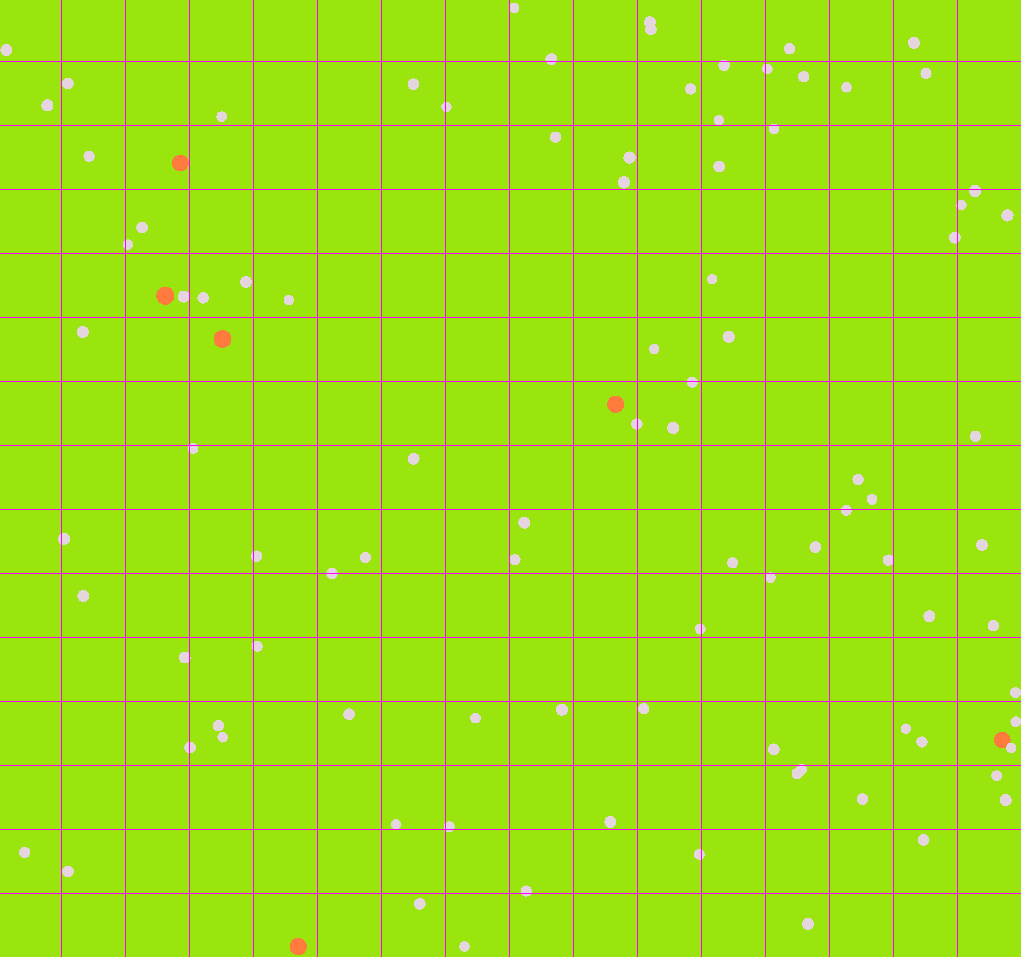
\includegraphics[scale=0.2]{figures/grid.png}
	\caption{Acceleration structure in grid}
\end{figure}

\begin{figure}[H]
	\centering
	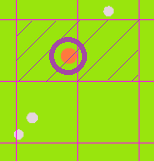
\includegraphics[scale=1]{figures/detection.png}
	\caption{Iterate on close cells}
\end{figure}

\end{document}